\documentclass{ctexart}
\usepackage{geometry}
\usepackage{listings}
\usepackage{textcomp}
\usepackage{graphicx}
\usepackage[hidelinks]{hyperref}
\usepackage{hyperref}
\usepackage{multirow}
\usepackage{amsmath,amssymb,amsfonts}
\usepackage[framed,numbered,autolinebreaks,useliterate]{mcode}
%记得用xelatex
% 导入首行缩进用的宏包
\usepackage{indentfirst}
\setlength{\parindent}{2em}
% 每行缩进两个汉字
\usepackage{url}
\setlength{\parindent}{0pt}
\setlength{\parskip}{18pt}
\title{\vspace{+4cm}\textbf{层次分析法的介绍与应用}}
\author{冯健齐}
\date{\today}
% //////////////////////////////////////////////////

\begin{document}

\maketitle
%目录
\newpage
\pagenumbering{Roman}
\setcounter{page}{0}
\tableofcontents
\newpage
\setcounter{page}{1}
\pagenumbering{arabic}
%标题

\section{问题背景}
\subsection{AHP的由来}
\setlength{\parindent}{2em}层次分析法(The Analytic Hierarchy Process)简称\textbf{AHP},是在20世纪70年代初期,美国匹兹堡大学运筹学家托马斯·塞蒂(T.L. Saaty)在为美国国防部研究“根据各个工业部门对国家福利的贡献大小而进行电力分配”的课题时提出的方法。它是一种应用网络系统理论和多目标综合评价方法,提出的一种层次权重决策分析方法。
\subsection{层次分析法原理}
\setlength{\parindent}{2em}层次分析法根据问题的性质和要求达到\textbf{总目标},将问题分解为不同的组成因素,并按照因素间的相互关联影响以及隶属关系将因素按不同层次聚集组合,形成一个多层次的分析结构模型,从而最终使问题归结为\textbf{最低层}(供决策的方案、措施等)相对于\textbf{最高层}(总目标)的相对重要权值的确定或相对优劣次序的排定。
\begin{figure}[h!]
    \centering
    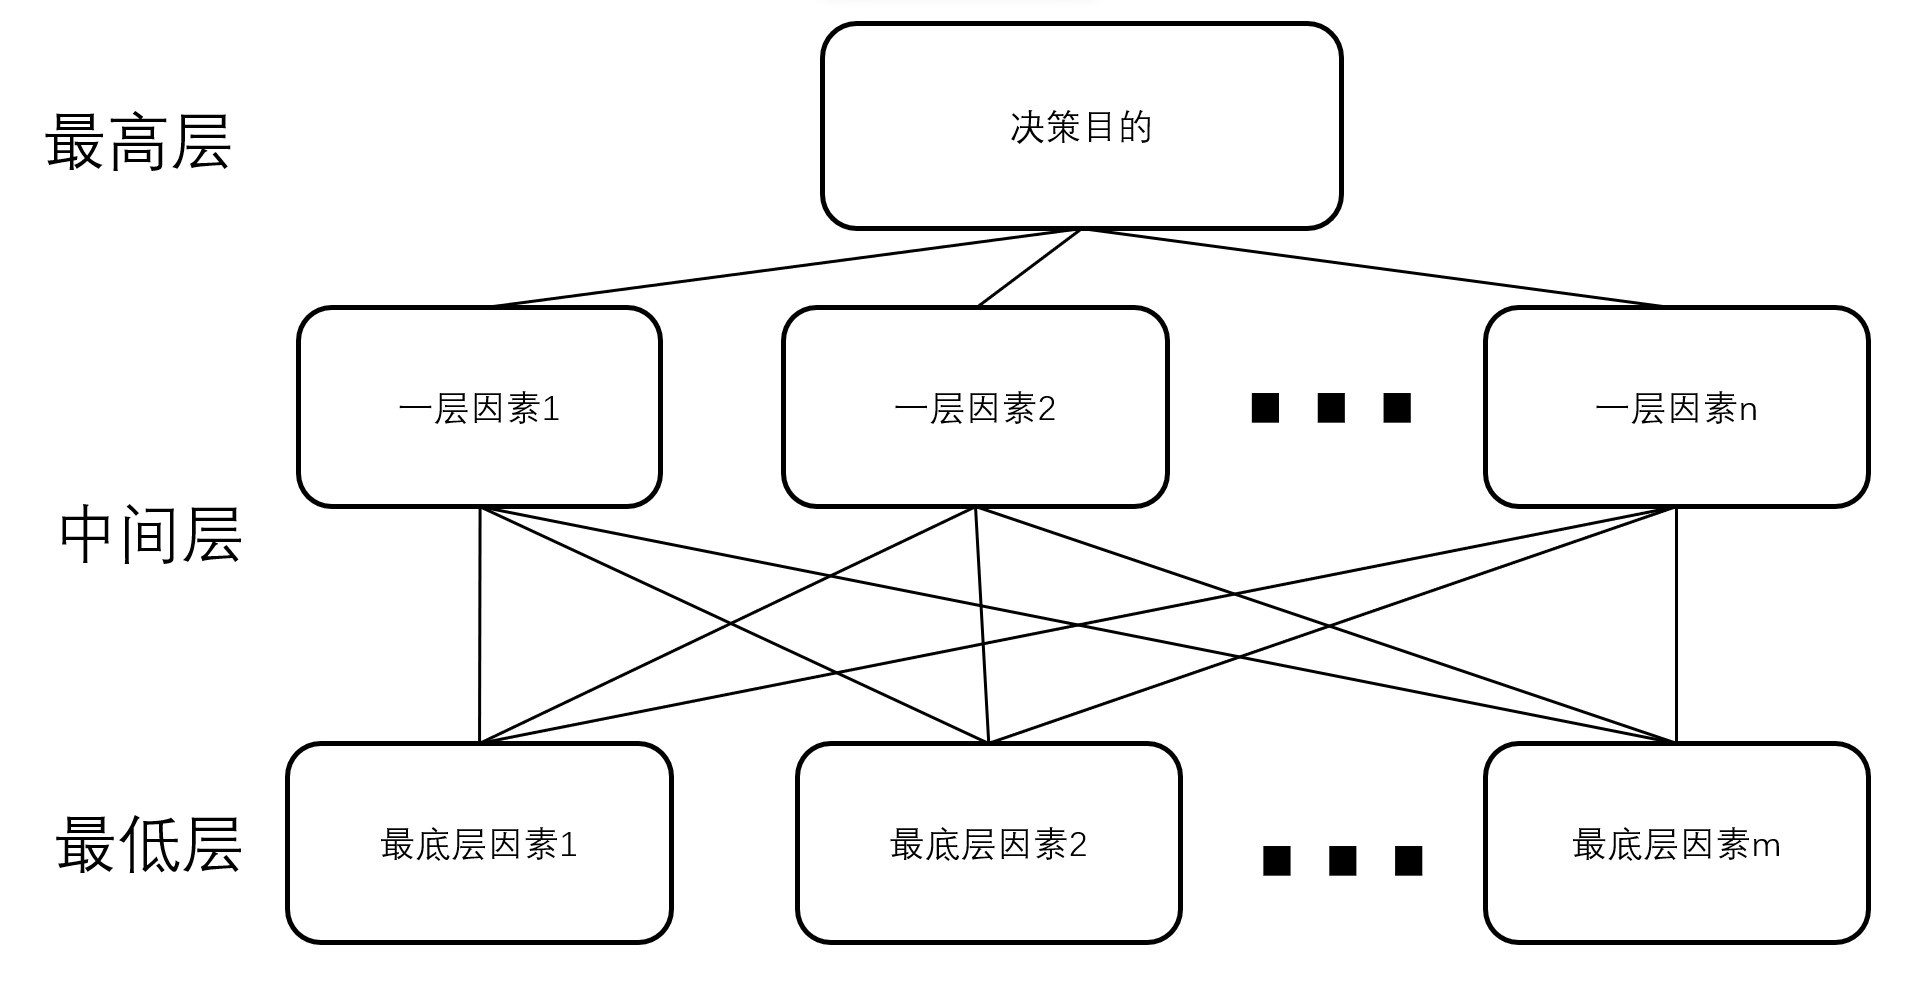
\includegraphics[width=0.9\textwidth]{001.JPG}
    \caption{各层之间的关系图}
\end{figure} 
%\textbf{最高层}:决策的目的、要解决的问题。\\
%\textbf{中间层}:考虑的因素、决策的准则。\\
%\textbf{最低层}:决策时的备选方案,也可以视为方案层。\\
%这里还是画图吧
\subsection{层次结构模型}
\setlength{\parindent}{2em}将决策的目标、考虑的因素(决策准则)和决策方案,按它们之间的相互关系分为最高层、中间层和最低层,绘出层次结构图。对于相邻的两层,称高层为目标层,低层为因素层。心理学家认为成对比较的因素不宜超过9个,即每层不要超过9个因素。下面给出判断矩阵元素$a_{ij}$的标度方法(见表\ref{表:1})。
\begin{table}[h!]
\centering
\begin{center}
 \begin{tabular}{||c c||} 
 \hline
 标度 & 含义\\ [0.5ex] 
 \hline\hline
 1 & 表示两个因素相比,具有同样的重要性\\ 
 \hline
 3 & 表示两个因素相比,一个因素比另一个因素稍微重要\\ 
 \hline
 5 & 表示两个因素相比,一个因素比另一个因素明显重要\\ 
 \hline
 7 & 表示两个因素相比,一个因素比另一个因素强烈重要\\ 
 \hline
 9 & 表示两个因素相比,一个因素比另一个因素极端重要\\  
  \hline
 2,4,6,8 & 上述两个相邻判断的中间值\\  
  \hline
 倒数 & 因素i与j比较的判断$a_{ij}$,则因素j与i的比较判断$a_{ji}=1/a_{ij}$\\  [1ex] 
 \hline
\end{tabular}
\end{center}
\caption{层次分析法中标度标度方法}
\label{表:1}
\end{table}\\

\setlength{\parindent}{2em}这样我们就可以得到一个判断矩阵(见表\ref{表:2}),其中的$A_{1},A_{2},A_{3}.\cdots.A_{n}$为底层因素,即决策层,要考虑的因素。$a_{ij}$表示$A_{i}$相对于$A_{j}$的重要程度。
\begin{table}[h!]
\centering
\begin{center}
 \begin{tabular}{|c|c|c|c|c|c|} 
 \hline
 Z & $A_{1}$ & $A_{2}$ & $A_{3}$ & $\cdots$ & $A_{n}$ \\
 \hline
 $A_{1}$  & $a_{11}$ & $a_{12}$ & $a_{13}$ & …… & $a_{1n}$ \\
 \hline
  $A_{2}$  & $a_{21}$ & $a_{22}$ & $a_{23}$ & …… & $a_{2n}$ \\
 \hline
  $A_{3}$  & $a_{31}$ & $a_{32}$ & $a_{33}$ & …… & $a_{3n}$ \\
 \hline
  $\vdots$ & $\vdots$ & $\vdots$ & $\vdots$ & $\ddots$ & $\vdots$ \\
 \hline
  $A_{n}$  & $a_{n1}$ & $a_{n2}$ & $a_{n3}$ & …… & $a_{nn}$ \\ [1ex] 
 \hline
\end{tabular}
\end{center}
\caption{判断矩阵}
\label{表:2}
\end{table}

\section{旅游地抉择问题}
\subsection{构造判断矩阵}
\setlength{\parindent}{2em}假设有三个心仪的旅游目的地$B_{1}$济南,$B_{2}$北戴河,$B_{3}$三亚。我们的选择标准有$A_{1}$景色,$A_{2}$费用,$A_{3}$居住,$A_{4}$饮食,$A_{5}$旅途,如何从中抉择出最佳的旅游目的地呢?

\begin{figure}[h!]
\centering
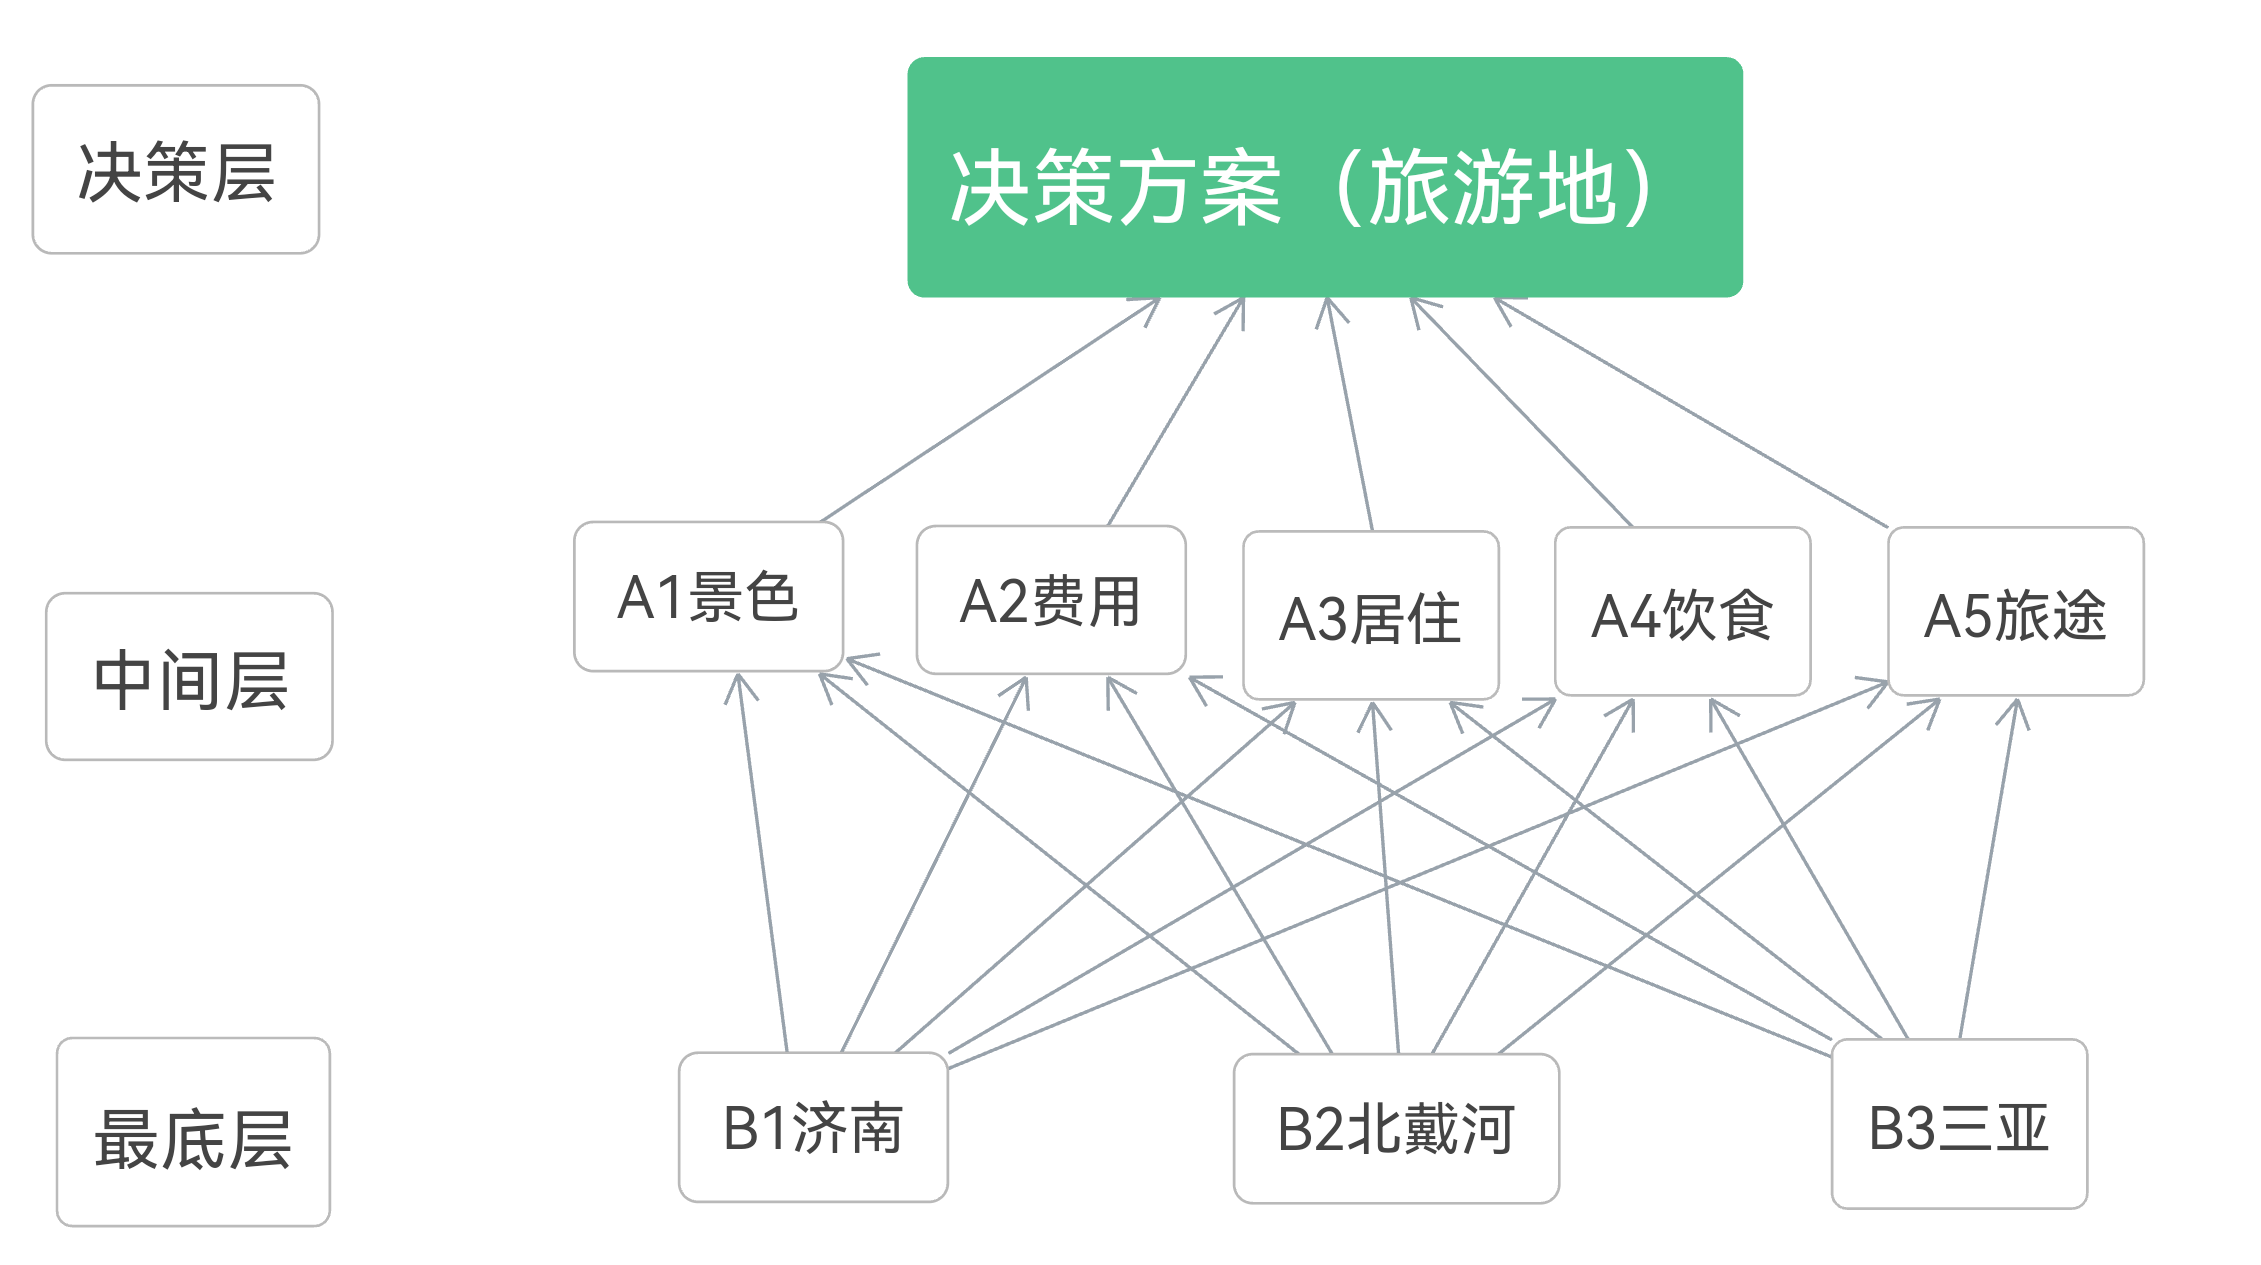
\includegraphics[width=0.8\textwidth]{002.png}
\caption{旅游问题抉择}
\end{figure}

%加入ABZ的图像

\setlength{\parindent}{2em}首先我们要根据自己的评判给出判断矩阵,得出下面的矩阵(见表3),例如其中$a_{14}=3$表示了选择旅游地时景色因素对比饮食因素来说稍微重要。\\

\begin{table}[h!]
\centering
\begin{center}
 \begin{tabular}{|c|c|c|c|c|c|} 
 \hline
 Z & $A_{1}$ & $A_{2}$ & $A_{3}$ & $A_{4}$& $A_{5}$ \\
 \hline
 $A_{1}$ & 1 & 1/2 & 4 & 3 & 3 \\
 \hline
  $A_{2}$ & 2 & 1 & 7 & 5 & 5 \\
 \hline
  $A_{3}$ & 1/4 & 1/7 & 1 & 1/2 & 1/3 \\
 \hline
  $A_{4}$ & 1/3 & 1/5 & 2 & 1 & 1 \\
 \hline
  $A_{5}$ & 1/3 & 1/5 & 3 & 1 & 1 \\
 \hline
\end{tabular}
\end{center}
\caption{旅游抉择判断矩阵}
\label{表:3}
\end{table}

\setlength{\parindent}{2em}在这里可以看到,$a_{23}=7$,但是根据$a_{21}$和$a_{13}$计算的话,$a_{23}$的值应为8,如果$a_{23}=a_{21} \times a_{13}$那么所有元素满足此运算,则称该成对矩阵为一致阵,一致阵中 A的最大特征根(值)为 $\lambda=n$ ,其余的 $n-1$ 个特征根均等于0,其最大特征值对应的特征向量可以作为比较上层因素的权向量。

\subsection{一致性判断}
 \setlength{\parindent}{2em}一般情况下,我们的矩阵不是一致阵,就与要进行一致性检验。那由于$\lambda$ 连续的依赖于$a_{ij}$ ,则 $\lambda$ 比$n$大的越多,A的不一致性越严重。用最大特征值对应的特征向量作为被比较因素对上层某因素影响程度的权向量,其不一致程度越大,引起的判断误差越大。因而可以用$\lambda-n$ 数值大小来衡量A的不一致程度。$CI=\frac{\lambda-n}{n-1}$;$CI=0$,有完全的一致性;$CI\rightarrow0$,有满意的一致性;CI越大,不一致越严重。
 下面进行平均随机一致性指标的计算。
 
 
\begin{lstlisting}{h!}
%一共有17个数,1,2,3……9,1/2,1/3……1/9
%按照1/17的平均概率均匀随机的抽取n^2个数,构成判断随机矩阵
%计算多次的平均值
clear
a=[9 8 7 6 5 4 3 2 1 1/2 1/3 1/4 1/5 1/6 1/7 1/8 1/9];
for k=2:50 %计算1到50阶的矩阵
    for n=1:10000 %对随机矩阵计算10000次
        A=ceil(17*rand(k)); %生成随机矩阵
        for i=1:k
            for j=i:k
                AA(i,j)=a(A(i,j));
                AA(j,i)=1/AA(i,j);
                AA(i,i)=1;
            end
        end
        BB=ones(k,k);
        for jj=1:k
            he=sum(AA(:,jj));
            BB(:,jj)=AA(:,jj)/he;
        end
        w=ones(k,1);
        for ii=1:k
            w(ii)=sum(BB(ii,:));
        end
        w=w./sum(w); %向量正规化
        L=sum((AA*w./(k.*w))); %正规化对应的最大特征值
        CI(n)=(L-k)/(k-1);
    end
    RI(k)=sum(CI)./n; %计算平均随机一致性指标
end
\end{lstlisting}


\begin{table}[h!]
\centering
\caption{随机一致性指标RI的数值}
\resizebox{\textwidth}{!}
{
 \begin{tabular}{|c|c|c|c|c|c|c|c|c|c|c|c|}
 \hline
 n & 1 & 2 & 3 & 4 & 5 & 6 & 7 & 8 & 9 & 10 & 11\\
 \hline
RI& 0 & 0 & 0.50453 & 0.90884 & 1.13579	&1.28758	&1.39181	&1.42631	&1.46843	&1.51110	&1.54223\\
\hline
\end{tabular}
}
\label{表:4}
\end{table}

\subsection{计算A对Z的权重}
在层次分析法中,矩阵的最大特征值对应的特征向量等于各个因素$A_{1},A_{2},A_{3},A_{4},A_{5}$对$Z$的影响权重,这一定理可以参考《层次分析法中特征向量法确定权重向量的理论》\cite{ref1},下面,我们计算A对Z的权重分析。

%matlab对za分析编程
\begin{lstlisting}
%输入矩阵的值
A=[1 1/2 4 3 3;
    2 1 7 5 5;
    1/4 1/7 1 1/2 1/3;
    1/3 1/5 2 1 1;
    1/3 1/5 3 1 1]
[n,n] = size(A);

%方法1:算术平均法求权重
SumA = sum(A);
SummA = repmat(SumA,n,1);
StandA = A ./ SummA;
disp('算术平均法求权重的结果为:');
%求行和之后再求平均
disp(sum(StandA,2)./n)

%方法2:几何平均法求权重
HangA = prod(A,2);%求行的乘积
JiheA = HangA .^ (1/n);%每行的几何平均
disp('几何平均法求权重的结果为:');
%求平均数
disp(JiheA ./ sum(JiheA))

%方法3:特征值法求权重
[V,D] = eig(A);
Max_eig = max(max(D));%求最大特征值
[r,c]=find(D == Max_eig , 1);
disp('特征值法求权重的结果为:');
%找到最大的特征值对应的特征向量
disp( V(:,c) ./ sum(V(:,c)) )

%下面计算一致性比例CR
CI = (Max_eig - n) / (n-1);
RI=[ 0 1e-10 0.50453 0.90884 1.13579 1.28758 1.39181 1.42631 1.46843 1.51110 1.54223];
% 这里n=2时,一定是一致矩阵,所以CI=0,为了避免分母为0,
%将这里的第二个元素改为了很接近0的正数

CR=CI/RI(n);
disp('一致性指标CI=');disp(CI);
disp('一致性比例CR=');disp(CR);
if CR<0.10
    disp('CR < 0.10,所以该判断矩阵A的一致性可以接受');
else
    disp('CR >= 0.10,该判断矩阵A需要进行修改');
end
\end{lstlisting}

可以计算得出以下各个特征值以及计算的一致性分析结果

\begin{table}[h!]
    \centering
    \begin{tabular}{|c|c|c|c|c|c|}
    \hline
         因素&  $A_{1}$ & $A_{2}$ & $A_{3}$ & $A_{4}$& $A_{5}$ \\
         \hline
         算数平均法 &0.2623 &0.4744 &0.0545 &0.0985 &0.1103\\
         \hline
         几何平均法 &0.2636 &0.4773 &0.0531 &0.0988 &0.1072\\
         \hline
         特征值法 &0.2636 &0.4758 &0.0538 &0.0981 &0.1087\\
         \hline
         CI & \multicolumn{5}{|c|}{0.0180}\\
         \hline
         CR & \multicolumn{5}{|c|}{0.0159}\\
         \hline
    \end{tabular}
    \caption{A对Z的一致性分析表格}
    \label{表:5}
\end{table}


可见,与标准的特征值法的计算结果相比,算术平均法和几何平均法计算出来的权重比例与特征值法相近。可以在简单计算时使用。由MATLAB我们得到了各个因素A对Z的影响权重,即$(0.2636,0.4758,0.0538,0.0981,0.1087)$,且随机一致性指标$CR=0.0159$ \textless $0.1$,通过一致性检验。


\subsection{计算B对A的权重}
下面是$B_{1},B_{2},B_{3}$分别对$A_{1},A_{2},A_{3},A_{4},A_{5}$的判断矩阵。例如,第一个矩阵是$B_{1},B_{2},B_{3}$对$A_{1}$的判断矩阵。
$$\begin{gathered}
\begin{pmatrix} 1 & 2 &5 \\ 1/2 & 1 & 2\\ 1/5& 1/2 &1\end{pmatrix}
\quad
\begin{pmatrix} 1 & 1/3 &1/8 \\ 3 & 1 & 1/3\\ 8& 3 &1\end{pmatrix}
\quad
\begin{pmatrix} 1 & 1 &3 \\ 1 & 1 & 3\\ 1/3& 1/3 &1\end{pmatrix}
\quad
\begin{pmatrix} 1 & 3 &4 \\ 1/3 & 1 & 1\\ 1/4& 1 &1\end{pmatrix}
\quad
\begin{pmatrix} 1 & 1 &1/4 \\ 1 & 1 & 1/4\\ 4& 4 &1\end{pmatrix}
\end{gathered}$$


下面对每个矩阵进行计算,得出各个因素的权重以及一致性指标。并且经过MATLAB计算,得出下面的权重(表6)。

\begin{lstlisting}
%录入各个矩阵的值
B=[1 2 5;1/2 1 2;1/5 1/2 1];%B1
B=[B [1 1/3 1/8;3 1 1/3;8 3 1]];%B2
B=[B [1 1 3;1 1 3;1/3 1/3 1]];%B3
B=[B [1 3 4;1/3 1 1;1/4 1 1]];%B4
B=[B [1 1 1/4;1 1 1/4;4 4 1]];%B5
for i=1:5
    A=B(:,[3*i-2:3*i]);
    disp(['B',num2str(i)])
    [n,n] = size(A);

%特征值法求权重
[V,D] = eig(A);
Max_eig = max(max(D));%求最大特征值
[r,c]=find(D == Max_eig , 1);
disp('特征值法求权重的结果为:');
%找到最大的特征值对应的特征向量
disp( V(:,c) ./ sum(V(:,c)) )

%下面计算一致性比例CR
CI = (Max_eig - n) / (n-1);
RI=[ 0 1e-10 0.50453 0.90884 1.13579 1.28758 1.39181 1.42631 1.46843 1.51110 1.54223];
% 这里n=2时,一定是一致矩阵,所以CI=0,为了避免分母为0,
%将这里的第二个元素改为了很接近0的正数
CR=CI/RI(n);
disp('一致性指标CI=');disp(CI);
disp('一致性比例CR=');disp(CR);
if CR<0.10
    disp('CR < 0.10,所以该判断矩阵A的一致性可以接受');
else
    disp('CR >= 0.10,该判断矩阵A需要进行修改');
end
end
\end{lstlisting}

\begin{table}[h!]
    \centering
    \begin{tabular}{c|c|c|c|c|c}
    \hline
         第二层&  $A_{1}$ & $A_{2}$ & $A_{3}$ & $A_{4}$& $A_{5}$ \\
         \hline
         A对Z权重 &0.2636 &0.4758 &0.0538 &0.0981 &0.1087\\
         \hline
         \multirow{3}{*}{B对A权重}
         &0.5954 &0.0819 &0.4286 &0.6337 &0.1667\\
         &0.2764 &0.2363 &0.4286 &0.1919 &0.1667\\
         &0.1283 &0.6817 &0.1429 &0.1744 &0.6667\\
         \hline
         CR &0.0055 &0.0015 &-2.2005e-15 &0.0091 &-8.8020e-16\\
         \hline
    \end{tabular}
    \caption{B对A的权重分析}
    \label{表:6}
\end{table}

可见,表格中的$CR$均 \textless $0.1$,均符合一致性指标,都通过一致性检验。



\subsection{计算B对Z的权重}
下面计算B对Z都权重影响,即对决策的影响程度。例如,$B1$对$Z$的影响程度为$0.5954 \times 0.2636 + 0.0819 \times 0.4758 + 0.4286 \times 0.0538 + 0.6337 \times 0.0981 + 0.1667 \times 0.1087$,下面计算出所有的影响值。

\begin{lstlisting}
%输入第二层矩阵的值
AA=[1 1/2 4 3 3;
    2 1 7 5 5;
    1/4 1/7 1 1/2 1/3;
    1/3 1/5 2 1 1;
    1/3 1/5 3 1 1];
[VV,DD] = eig(AA);
Max_eigAA = max(max(DD));%求最大特征值
[rr,cc]=find(DD == Max_eigAA , 1);
%找到最大的特征值对应的特征向量
wA=VV(:,cc) ./ sum(VV(:,cc));

%录入第三层矩阵的值
B=[1 2 5;1/2 1 2;1/5 1/2 1];%B1
B=[B [1 1/3 1/8;3 1 1/3;8 3 1]];%B2
B=[B [1 1 3;1 1 3;1/3 1/3 1]];%B3
B=[B [1 3 4;1/3 1 1;1/4 1 1]];%B4
B=[B [1 1 1/4;1 1 1/4;4 4 1]];%B5
wB=[];
for i=1:5
    A=B(:,[3*i-2:3*i]);
    [V,D] = eig(A);
    Max_eig = max(max(D));%求最大特征值
    [r,c]=find(D == Max_eig , 1);
    %找到最大的特征值对应的特征向量
    wB=[wB V(:,c) ./ sum(V(:,c))];
end
disp('第一层各个权重值');
disp(wA);
disp('第二层各个权重值');
disp(wB);

%计算各个因素的总权重
E=[];
for j=1:3
    W=wB(j,:)*wA;
    E=[E;W];
end
disp('第二层对总方案的权重');
disp(E);
\end{lstlisting}

    
得到三个旅游景点$B_{1}$济南,$B_{2}$北戴河,$B_{3}$三亚,对方案-决定旅游去处的权重为\\(0.2993,0.2453,0.4554),即三亚 \textgreater 北戴河 \textgreater 济南。
    
\section{更多介绍}
\subsection{AHP的优化}
AHP方法只适合多层之间各个的权重关系,但实际上,往往要素之间的影响并非简单的层级关系,往往是以网络形式存在,为了更好的分析评价这类模型,其发明者T.L.Saaty在AHP的基础上提出了网络分析法(Analytic Network Process)简称为ANP。ANP是AHP方法的延伸,两者的理论都是基于成对比较决策矩阵而来。

\subsection{AHP的推广}
后面,还有更加优化的方法,如决策与实验室方法-DEMATEL(Decision-making Trial and Evaluation Laboratory)\cite{ref2}.该方法的优化之处在于,AHP, ANP的前提都是两两比较的结果互相为倒数,但是这只是凭经验规则的定制,并没有数理逻辑,于是DEMATEL和D-ANP方法就诞生了。DEMATEL中把元素之间的关系视为一个带权值的有向图。同样计算判断矩阵的各种值,由于抛弃了互为倒数的限制,DEMATEL方法可以得到各个要素的影响度,被影响度,中心度,原因度。

\begin{thebibliography}{99}  

\bibitem{ref1}\href{https://max.book118.com/html/2019/0103/8106046045001143.shtm}{黄德所,张俊学,层次分析法中特征向量法确定权重向量的理论,1998中国控制与决策学术年会论文集}
\bibitem{ref2}\href{http://www.huaxuejia.cn/ism/dematelintro.php}{决策与实验室DEMATEL方法}
\addcontentsline{toc}{section}{参考文献}
\end{thebibliography}

\end{document}
